\documentclass[11pt]{article}
\usepackage[margin=0.8in]{geometry}
\usepackage{graphicx,booktabs,amsmath,hyperref}
\hypersetup{colorlinks=true,urlcolor=blue}
\title{Observational Reboot: Conditional SMICA Pilot and Research Programme}
\author{HTT observational research}\date{14 October 2026}
\begin{document}\maketitle
\begin{abstract}
We executed a source-bound, retrospective exploratory low-mode SMICA experiment,
a finite-null calibration utility, and a local/global response laboratory.
The global rank is 129/241 = 0.535270. It is conditional on a declared delivered-simulation
model, not a confirmatory physical Planck null probability or a Bianchi result.
The continuation covers all feasible analyses in the existing theory, code and data.
\end{abstract}
\section{Executed SMICA experiment}
The K1 NSIDE64 cache was verified against its accepted byte-identity gate.
One observation and 300 separately delivered signal/noise pairs use the identical
38,413-pixel mask and simultaneous 36-column $\ell=0,\ldots,5$ fit. Each simulation
component is used once. Training uses 60 pairs; calibration uses the other 240.
The four features are squared norms of retained real harmonic coefficients divided
by $2\ell+1$. These are selected-sky fitted power summaries in $\mu$K$^2$, not
certified unbiased full-sky power estimates.
\begin{center}\begin{tabular}{rrrr}\toprule
$\ell$ & Power summary & Marginal rank & Max-adjusted rank\\\midrule
2 & 226.451 & 0.1120 & 0.5353 \\
3 & 402.198 & 0.5353 & 0.9461 \\
4 & 239.881 & 0.5685 & 0.9751 \\
5 & 291.639 & 0.2697 & 0.6971 \\
\bottomrule\end{tabular}\end{center}
The score is the maximum of four absolute departures standardized using training
only. There are 128 exceedances among 240 calibration rows, giving 129/241 = 0.535270.
The rank floor is $1/241$. The 95\% Clopper--Pearson interval $[0.468058,0.597775]$
concerns the IID conditional null-tail probability, not the realized discrete rank.
\begin{figure}[ht]\centering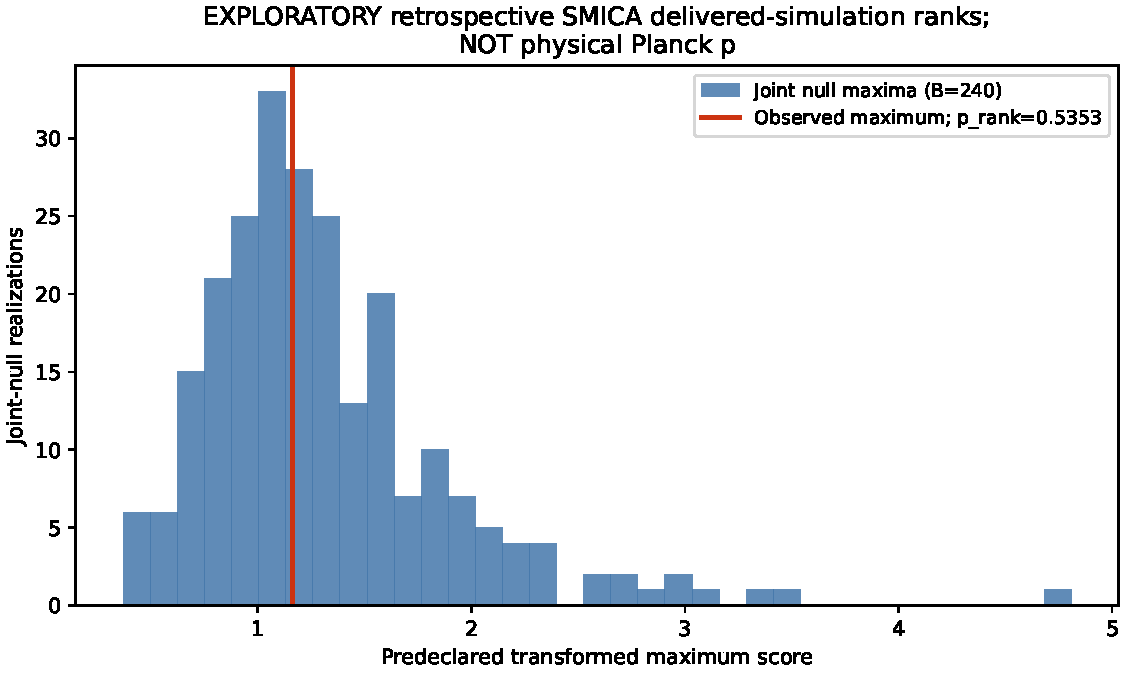
\includegraphics[width=.9\linewidth]{docs/observational_reboot_20261014/results/smica_pilot/joint_null_maximum.pdf}\caption{Actual SMICA, retrospective conditional delivered-simulation rank. The feature family and current split were fixed before this run, after historical examination of this sky.}\end{figure}
\clearpage
\section{Interpretation and historical comparison}
Planck's release describes independent noise/systematic simulations and linear
separate propagation at fixed actual-data weights. The official plancklens library
adds delivered signal and noise maps. This supports our addition recipe, while
observed-simulation exchangeability, foreground residuals, fixed weights and
systematic means remain physical-model obligations. We did not subtract the
simulation mean as an assumed observed bias. The OLS identity residual near
$2.1\times10^{-15}$ verifies algebra, not omitted-mode leakage.

The old K1 rank 0.039 used another processing/statistic family and 999 signals with
300 cyclically reused noise draws. Archive 0.078/0.079 were posterior-predictive
discrepancies combining dipole, CF4 and scalar D2/D3 summaries. The R8 finite-rank enclosures were synthetic
pools. None is an interchangeable predecessor of this result. The legacy review
also identifies $D_\ell/C_\ell$ and STF normalization differences.

\section{Finite-null implementation checks}
A fixed-$B=999$, 1000-repetition correlated-feature experiment returned a 0.060
global rejection rate; its 95\% binomial interval is [0.04610,0.07656]. Choosing the
smallest unadjusted marginal rank returned 0.145. The campaign is conditional on one fixed independent training sample. This tests the declared synthetic
procedure, not empirical Planck calibration. Tests exercise exact inclusive ties,
binomial interval coverage, disjoint training, same-sky rejection and projection.
\begin{figure}[ht]\centering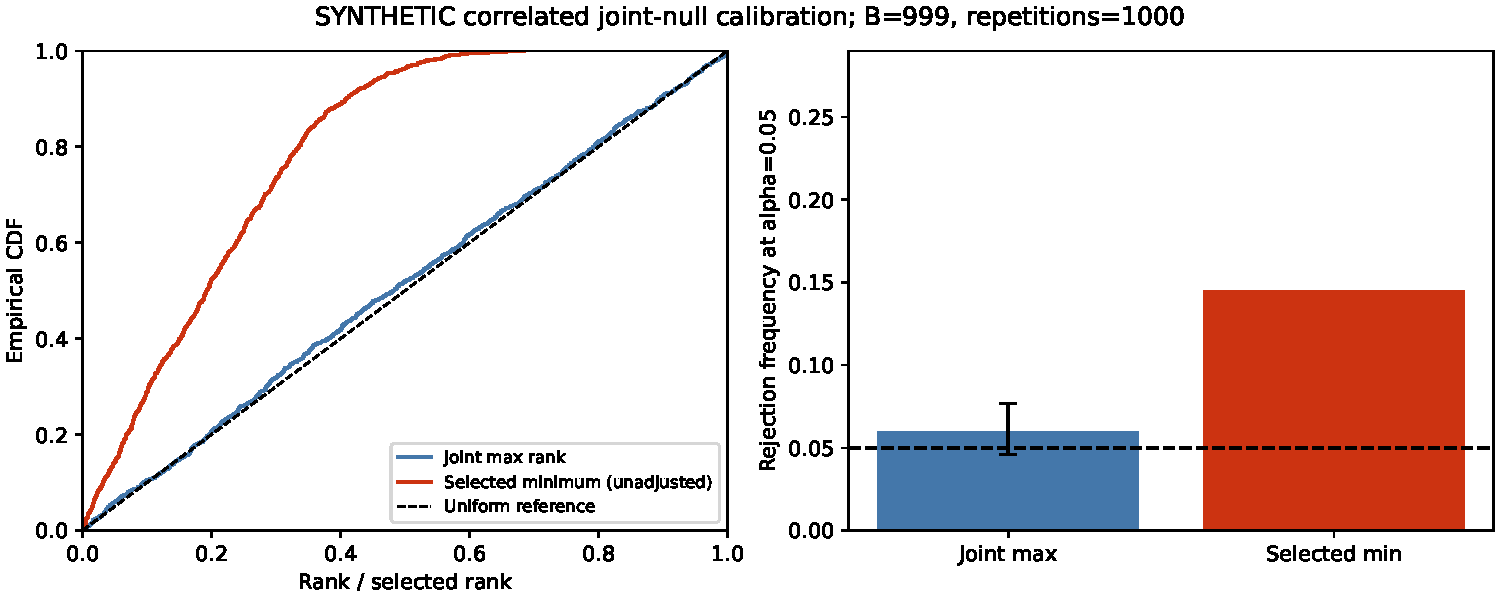
\includegraphics[width=.93\linewidth]{docs/observational_reboot_20261014/results/synthetic_calibration/synthetic_calibration_campaign.pdf}\caption{Synthetic calibration experiment. Error rates apply to the specified correlated Gaussian generator; the Planck physical law is a separate obligation.}\end{figure}
\clearpage
\section{Local/global response and continued analysis}
For a declared linear Gaussian model $y=B\beta_L+G\beta_G+\epsilon$, nuisance
projection after covariance whitening gives the conditional information
$G_w^T(I-P_{B_w})G_w$. In the synthetic laboratory the constant response has rank 0,
the specified depth response has rank 3, and free shell nuisance gives rank 0.
Full rank can still be arbitrarily weakly informative. Nuisance-column normalization
preserves its span under parameter-unit changes.
\begin{figure}[ht]\centering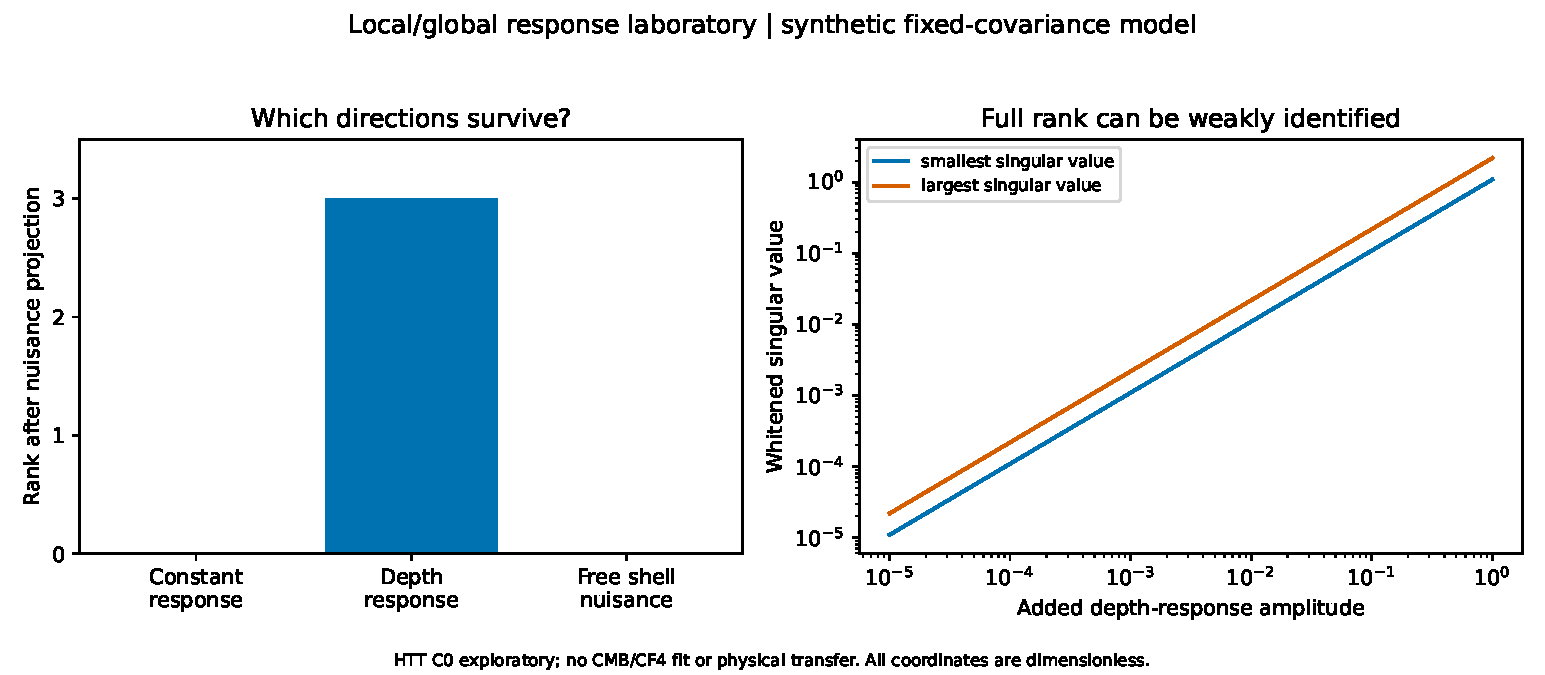
\includegraphics[width=\linewidth]{docs/observational_reboot_20261014/results/response_laboratory/response_identifiability.pdf}\caption{Specified dimensionless response model with known covariance. This is not an observed velocity or global-tilt estimate.}\end{figure}
The theory note derives endpoint boost/STF response, a nuisance quotient,
two-shell discrimination, shared-sky covariance and a restricted Bianchi-I history.
Small Wolfram and NumPy checks are not four-axis CAS admission or a native atlas.

The 23-card DAG and 20-opportunity inventory cover SMICA, physical dipole and
local/global response, CF4/SDSS depth laws, DESI/Union3/JWST distances, released
lensing and spectra, and polarization controls. Codex must assign concrete goals,
execute and review each ready analysis, publish generated figures/reports and
continue. Missing native inputs block their branch only. Capability discovery
continues beyond this sampled inventory; the present completed unit is RB00.

\section*{Source and reproduction pointers}
Full numerical input hashes and source paths: \texttt{report.json}.
Commands, failures and targeted repairs: the sibling \texttt{evidence} directory.
Independent review, goal queue and copyable handoff are linked from the package README.
Primary source context: Planck 2018IV, \href{https://arxiv.org/abs/1807.06208}{arXiv:1807.06208};
Planck 2018VII, \href{https://arxiv.org/abs/1906.02552}{arXiv:1906.02552};
Dai--Chluba, \href{https://arxiv.org/abs/1403.6117}{arXiv:1403.6117};
Roldan et al., \href{https://arxiv.org/abs/1603.02664}{arXiv:1603.02664};
Saadeh et al., \href{https://arxiv.org/abs/1605.07178}{arXiv:1605.07178}.
See the source registry for exact read scope and methodological limits.
\end{document}
